\section{Detalhamento do Problema e justificativa} % (fold)
\label{sec:detalhamentoProblema}

O campus do Gama da Universidade de Brasília (figura 1), construído entre os anos de 2009 a 2011 , localizado na Área Especial de Indústria Projeção A, UnB- DF- 480- Gama Leste, Brasília-DF, possui área total de 335074 m$^2$, com área construída de aproximadamente 16009 m$^2$, sendo projetado para abrigar, no total, cinco cursos de engenharia, sendo eles de Aeroespacial, Automotiva, Eletrônica, Energia e Software.

\begin{figure}[H]
	\centering
	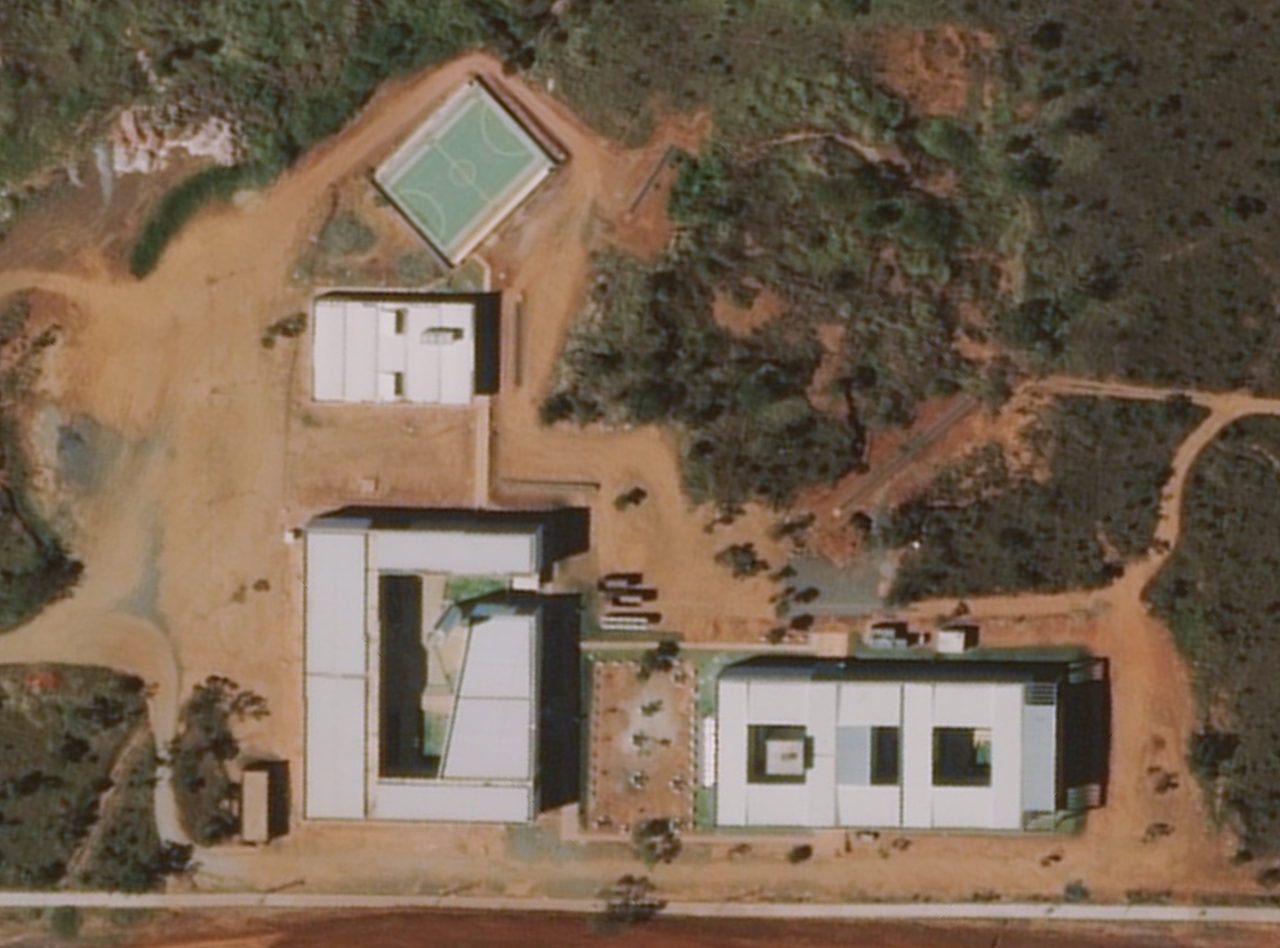
\includegraphics[width=0.6\textwidth]{figuras/fga1}
	\caption[Vista aérea do campus UnB Gama: área construída]{Vista aérea do campus UnB Gama: área construída~\cite{mapa1}}
	\label{img:fga1}
\end{figure}


Em 2013, segundo informações do DaEng, sete meses após o início da gestão do Diretório Acadêmico do Gama, iniciaram-se medidas para a implementação do cercamento do campus. Contudo, mediante a falta de documentos legais, como licenciamento ambiental e demarcação de terras, o processo de licitação teve de ser adiado e, somente em meados do ano de 2015 as obras foram iniciadas.

Diante disso, durante os anos de 2012 até os dias atuais, muitos alunos, professores e comunidade em geral que frequentam a Faculdade do Gama vêm enfrentando uma rotina de roubos a carros na área do estacionamento do campus, cujo principal fator seria a da falta de um cercamento, com guaritas, que possibilitassem o controle de pessoas que acessam o local. Os relatos dos alunos que foram vítimas dos furtos alegam, em sua maioria, terem sido levados o estepe e dispositivos de som.

Dessa forma, foi elaborado um diagrama de espinha de peixe para avaliar os principais motivos pelos quais a comunidade da Faculdade do Gama sente-se insegura. Os problemas elencados apresentam estreita correlação com a falta de estrutura do campus e cercamento do local, ocasionando, por exemplo, a fuga rápida do indivíduo infrator. A falta de câmeras externas, a ausência de policiamento e a localização isolada do campus também facilitam ações criminosas.

\begin{figure}[H]
	\centering
	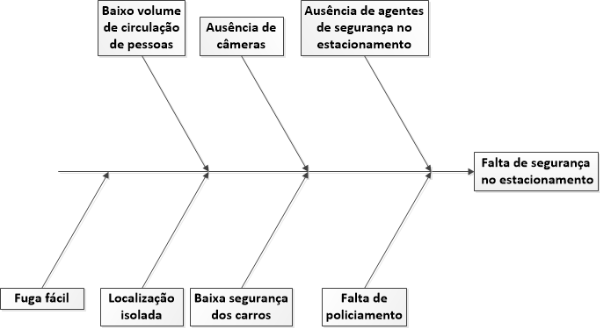
\includegraphics[width=0.6\textwidth]{figuras/fishbone}
	\caption{Principais motivos responsáveis pela falta de segurança no estacionamento do campus FGA.}
	\label{img:fishbone}
\end{figure}

Também, como maneira de obter alguns dados referentes à mobilidade de alunos, professores e comunidade até o campus, o Grupo 1 da disciplina Projeto Integrador 1 decidiu aplicar uma pesquisa sobre o meio de transporte utilizado para descolamento residência-campus,   quantas vezes o veículo foi roubado, se o indivíduo prestou alguma queixa formal (boletim de ocorrência) e o(s) ano(s) do ocorrido, caso este utilize automóvel para locomoção.

\begin{figure}[H]
	\centering
	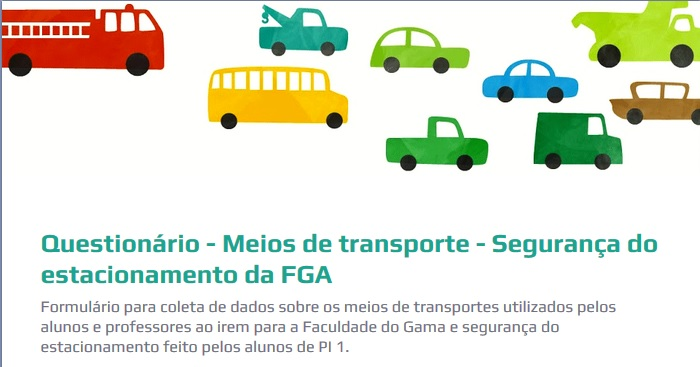
\includegraphics[width=0.6\textwidth]{figuras/questionario}
	\caption{Questionário sobre mobilidade e segurança do campus.}
	\label{img:questionario}
\end{figure}

A pesquisa foi elaborada no aplicativo Google Drive - Formulários e publicada no período do dia 02 de agosto de 2015 ao dia 29 de agosto do mesmo ano no grupo destinado aos alunos e professores da UnB-Gama, na rede social Facebook. Durante este período, 93 pessoas responderam às seis questões propostas no questionário, resultando nos dados apresentados nos gráficos a seguir:

\begin{figure}[H]
	\centering
	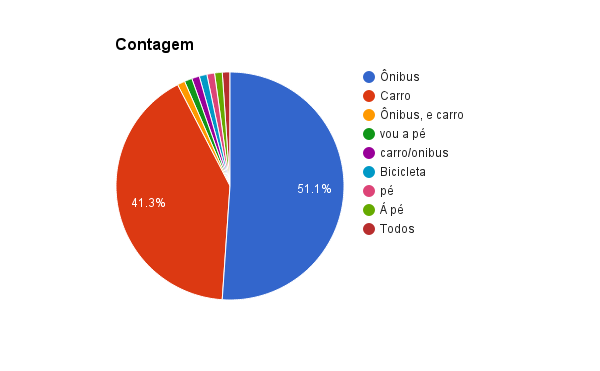
\includegraphics[width=0.6\textwidth]{figuras/resultadoquestionario}
	\caption{Pesquisa de mobilidade dos alunos da FGA: meios utilizados para deslocamento residência-FGA}
	\label{img:resultadoquestionario}
\end{figure}

O gráfico apresentado na Figura \ref{img:resultadoquestionario} apresenta a distribuição, no espaço amostral, dos meios  de transporte utilizados. Mais da metade dos alunos (51,1\%) utilizam apenas ônibus para locomoção, 41,3\% utilizam apenas o carro como meio de transporte, e os 7,6\% restantes se locomovem a pé, de bicicleta, de ônibus ou de carro. Apresenta-se, então, uma significativa frota de carros diária no campus, demandando maiores investimentos para segurança destes bens.

O gráfico apresentado na Figura \ref{img:resultadoquestionario2}, gerado pelo programa \emph{Numbers}, apresenta, de acordo com a amostra total de usuários de carros, que 11 carros foram furtados e que, deste total, 9 pessoas apresentaram queixa formal, ou seja, boletim de ocorrência. O período dos furtos foi de 2010 a 2015.

\begin{figure}[H]
	\centering
	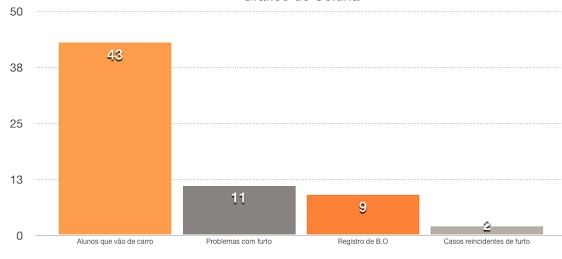
\includegraphics[width=0.6\textwidth]{figuras/resultadoquestionario2}
	\caption{Pesquisa de mobilidade de alunos da FGA: índices de furtos e registros de boletins de ocorrência no período dos anos de 2010 a 2015}
	\label{img:resultadoquestionario2}
\end{figure}

Dessa maneira, baseando-se nos dados coletados e avaliando os riscos nos quais os alunos estão submetidos, há, então, a necessidade de se projetar  um sistema que, em conjunto com a segurança do campus, possa realizar o monitoramento  da área do estacionamento, de maneira eficiente, e fluxo de pessoas, com o objetivo de aumentar o controle de entradas e saídas de veículos e pessoas no campus e alertar às autoridades responsáveis, em casos de furtos, em tempo hábil para que as medidas necessárias sejam tomadas.

% section section_name (end)

\section{Objetivos} % (fold)
\label{sec:objetivos}

  \subsection{Objetivos Gerais} % (fold)
  \label{sub:objetivos_gerais}

  O objetivo geral do projeto é desenvolver um sistema que potencialize a segurança já existente no estacionamento do campus da UnB Gama, de modo que este monitore a circulação de carros e movimentações de pessoas, identificando possíveis situações de risco e acionando, com o auxílio de um operador na estação de solo, local para onde serão transmitidas as imagens, as entidades responsáveis pela segurança do campus da Faculdade do Gama para coibir o furto.

  \subsection{Objetivos Específicos} % (fold)
  \label{sub:objetivos_espec_ficos}

% section Objetivos (end)

\section{Definição do Escopo} % (fold)
\label{sec:defini_o_do_escopo}


  O Sistema Unificado de Monitoramento irá fazer o monitoramento de toda a área externa do campus da UnB Gama, em específico da área do estacionamento, que é de 16100 m$^2$ (delimitada em azul na Figura \ref{img:fga2}).

  \begin{figure}[H]
  	\centering
  	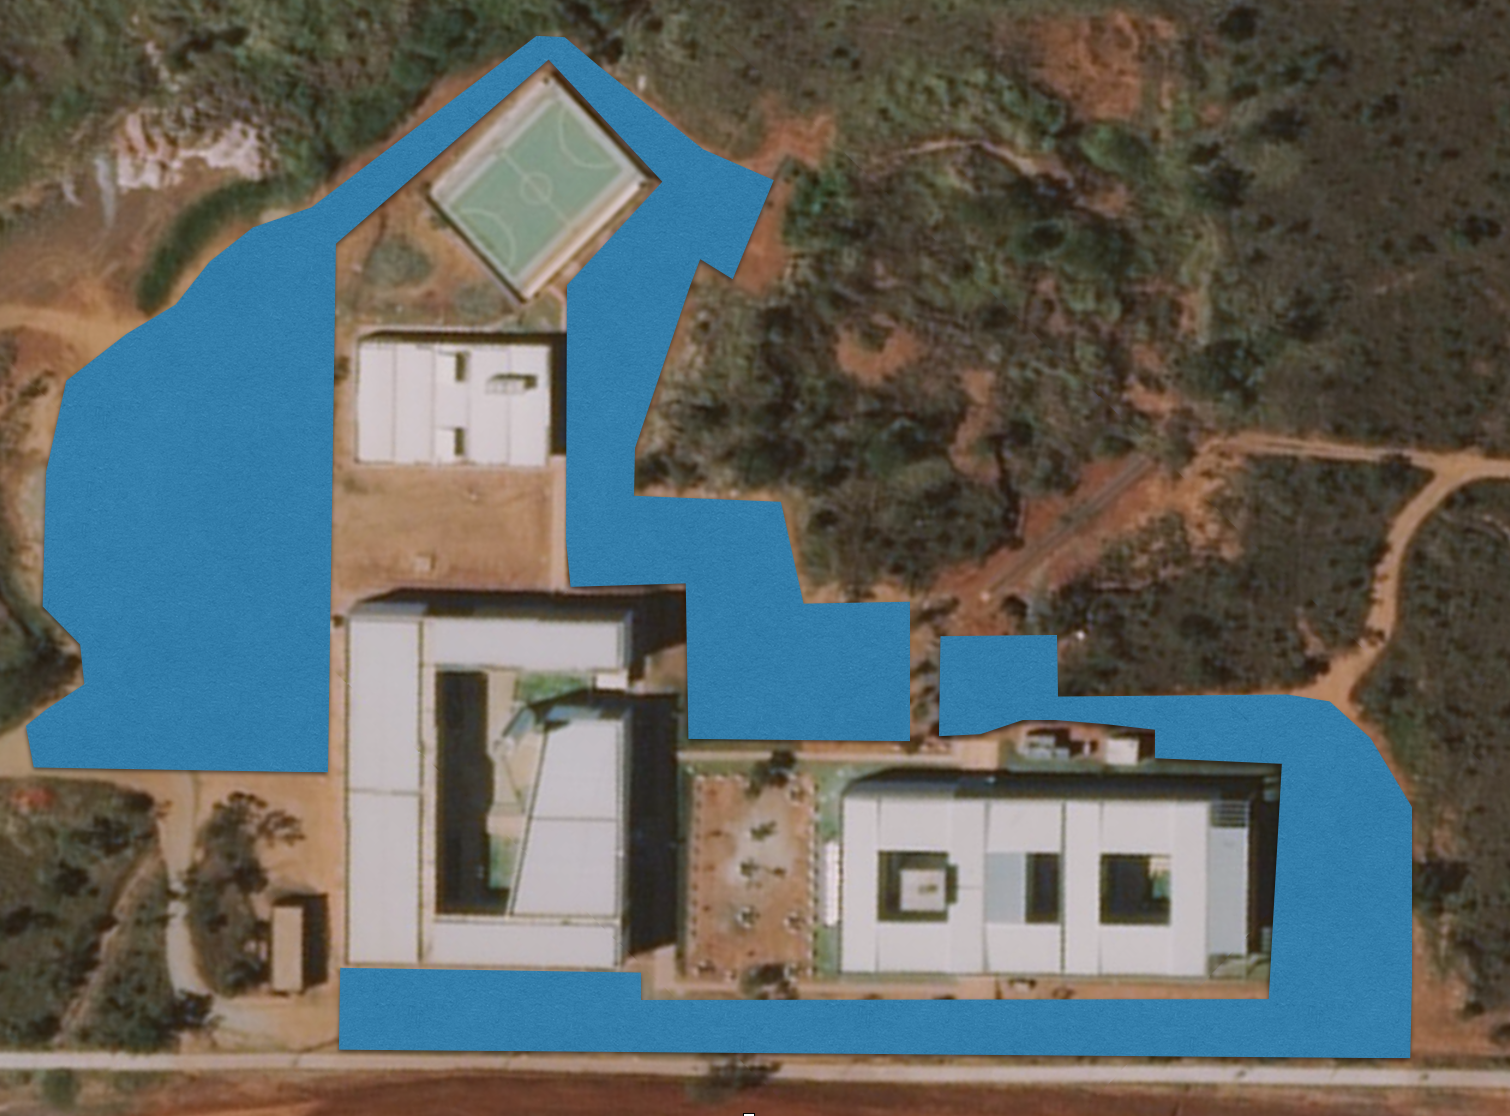
\includegraphics[width=0.6\textwidth]{figuras/fga2}
  	\caption[Vista aérea do Campus FGA:  áreas de estacionamento do campus]{Vista aérea do Campus FGA:  áreas de estacionamento do campus~\cite{mapa1}}
  	\label{img:fga2}
  \end{figure}

  O monitoramento será exclusivamente externo, como já definido, e os balões estarão localizados nos térreos dos prédios UED, UAD E RU, de forma que toda a área seja monitorada e não haja pontos cegos. Dessa forma, o monitoramento interno dos prédios não estará incluído no escopo do projeto, pois o objetivo é o monitoramento do fluxo de pessoas e carros no estacionamento do campus, e este será de responsabilidade total da instituição.

  O funcionamento do balão será baseado na captação e processamento de imagens que, posteriormente, serão transmitidas para uma estação de solo, que irá autenticar as informações e, com o auxílio de um operador funcionário da instituição, estas imagens serão interpretadas e, se identificados padrões de atividades caracterizadas como suspeitas ou de furto, as entidades responsáveis pela Faculdade do Gama serão acionadas. A opção de acionamento da polícia não entrará no escopo do projeto, pois o SUM é um mecanismo interno da UnB-Gama e que visa apenas a identificação de possíveis atividades suspeitas e rápida tomada de decisão pela segurança do campus. É importante salientar que não será feita a identificação facial da pessoa que está realizando a atividade suspeita.

  O sistema identificará todas as áreas do estacionamento em que houver atividade suspeita, alertando visualmente o operador do sistema e informando o grau de risco da situação identificada. O sistema utilizará os seguintes fatores para calcular o risco de furto numa determinada área:

  \begin{itemize}
    \item Presença de pessoas nas áreas delimitadas como estacionamentos por tempo maior que 30 segundos.
    \item Aproximação de um raio de 2 metros de um grupo de automóvel por período superior a 5 segundos com pouca movimentação.
    \item Sair do campo de visão da câmera por mais de 5 segundos estando próximo de um automóvel.
    \item Tocar constantemente em um automóvel e em um curto espaço de tempo sem adentrar no mesmo.
  \end{itemize}

  Os fatores elencados acima terão um valor específico que, em conjunto com outros fatores, definirão as atividades com risco de furto baixo, médio ou alto.

  O operador recebendo os alertas visualmente nas telas de monitoramento, conseguirá identificar quais áreas merecem mais atenção quanto à sua observação, sendo seu dever certificar se a atividade suspeita necessita de intervenção por parte da segurança do campus ou se é apenas um alarme falso.

  Devido ao custo elevado e incertezas inerentes ao uso de inteligência artificial na identificação de crimes em lugares de grande movimentação e sem controle de fluxo de pessoas, decidiu-se por utilizar este sistema híbrido que concilia a tomada de decisão humana com a praticidade, facilidade e rapidez na identificação de atividades suspeitas feitos por um sistema inteligente, mas não autônomo.

  As câmeras a serem utilizadas para monitoramento, e que estarão acopladas à \emph{payload}, serão de longo alcance e infravermelho.  As câmeras de longo alcance deverão captar imagens com qualidade suficiente para identificação de movimentação suspeita, abrangendo toda a área do estacionamento. As câmeras de \emph{leds} infravermelhos terão como objetivo o monitoramento noturno.

  O SUM será composto pelo conjunto de balões cativos posicionados em locais estratégicos da área externa do campus, especificamente nos terraços dos três prédios do campus, para a melhor visualização das movimentações nas áreas do estacionamento. Os balões irão funcionar até 25 metros de altitude, com capacidade para levantar 10 kg de carga útil, incluindo cabo de energia. O sistema irá funcionar 24/7 (24 horas por dia, 7 dias por semana) devido às várias atividades fora do período de aulas, que é das 8:00 às 18:00 horas. Por exemplo, concursos públicos, aulas da UnB Idiomas, eventos culturais, etc. Contudo, o sistema não irá operar quando houver condições adversas de tempo, como chuva intensa, e tormenta elétrica, devido a possibilidade de danos ao equipamento.

  O monitoramento a noite será feito com o uso de câmeras de leds infravermelho, como já definido anteriormente. Todavia, avaliando as condições visuais, a altitude do balão e a distância que este estará do estacionamento, pois os \emph{leds} não terão capacidade  de identificar atividades suspeitas nas condições supracitadas, sendo necessário a utilização de um sistema de iluminação acionado quando houver detecção de movimento. No entanto, a instalação dos postes não faz parte do escopo deste projeto.

\section{Metodologia de Gerenciamento de Projeto} % (fold)

  Para início do projeto, foi elaborada uma análise de requisitos a partir de um documento de visão. O documento de visão desenvolvido fez o uso do diagrama de espinha de peixe para elencar as principais causas da insegurança do campus, definindo em seguida os requisitos a serem trabalhados para a elaboração de uma Estrutura Análitica do Projeto (EAP).

  Para a realização do desenvolvimento do projeto SUM, foi necessário estruturar uma metodologia de trabalho em que todos os integrantes do grupo possam interagir e apresentar resultados de maneira rápida e eficaz. E a metodologia que mais se adequa à dinâmica do projeto é o SCRUM.

  O SCRUM é uma metodologia ágil para gestão de projetos na área de \emph{software}, que, no contexto da disciplina de Projeto Integrador 1, foi adaptado para o gerenciamento de projetos de engenharia.
  No SCRUM, as funcionalidades do produto são organizadas em dois artefatos, o \emph{backlog} de produto e o \emph{backlog} da \emph{sprint}. O \emph{backlog} do produto possui uma visão mais abrangente da funcionalidade, enquanto que no \emph{backlog} da \emph{sprint}, essas funcionalidades são refinadas e melhor descritas.

  Os seguintes itens do \emph{backlog} do SUM foram planejados:

  \begin{itemize}
    \item Monitoramento aéreo do estacionamento da FGA.
    \item Facilidade de instalação e manutenção.
    \item Identificação de problemas de funcionamento interno.
    \item Transmissão de dados para estação em solo.
    \item Identificação de atividade suspeita por meio de inteligência artificial.
    \item Emissão de alerta de atividade suspeita quando identificada.
    \item Armazenamento de dados coletados por grandes períodos.
    \item Capacidade de funcionamento temporário quando houver falha de alimentação  energética.
    \item Garantia de cobertura do monitoramento de toda a área do estacionamento.
    \item Capacidade de controlar altura em relação ao solo.
\end{itemize}

  O backlog de produto será refinado durante as \emph{sprints}, a fim de cumprir as expectativas dos pontos de controle definidos na disciplina de Projeto Integrador 1. Nesse sentido, cada ponto de controle será contemplado por duas \emph{sprints}: a primeira \emph{sprint} cobrirá metade dos itens do backlog de produto com o enfoco necessário para o Ponto de Controle 1; e a segunda \emph{sprint}, cobrirá o restante dos itens do backlog de produto.

  A tabela \ref{tab:enfoque_pc} delimita o enfoco de cada ponto de controle:

  \begin{table}[H]
  \centering
  \begin{tabular}{|p{4cm}|p{12cm}|}
  \hline
  Ponto de Controle & Enfoque                                                                                      \\ \hline
  1                 & Definir o escopo dos itens do \textit{Backlog} de produto , realizar revisão bibliográfica \\ \hline
  2                 & Refinar soluções técnicas, modelagem da solução                                              \\ \hline
  3                 & Análise de viabilidade econômica                                                             \\ \hline
  \end{tabular}
  \caption{Enfoque por ponto de controle}
  \label{tab:enfoque_pc}
  \end{table}

	A partir do \emph{backlog} do produto foi elaborada a Estrutura Analítica do Projeto (EAP), com o objetivo de subdividir as áreas de pesquisa para desenvolver o projeto. Foram elencadas cinco grandes áreas de pesquisa, que, com o progresso das revisões bibliográficas, puderam ser subdivididos em outros níveis específicos. As áreas de pesquisa não foram subdivididas em engenharias, pois muitos tópicos de pesquisa são integrados e isto limitaria a interação de cada aluno.

	As grandes áreas de pesquisa são: logística, estrutura, eletrônica embarcada, estação de solo e sistema aéreo.

  \begin{figure}[H]
  	\centering
  	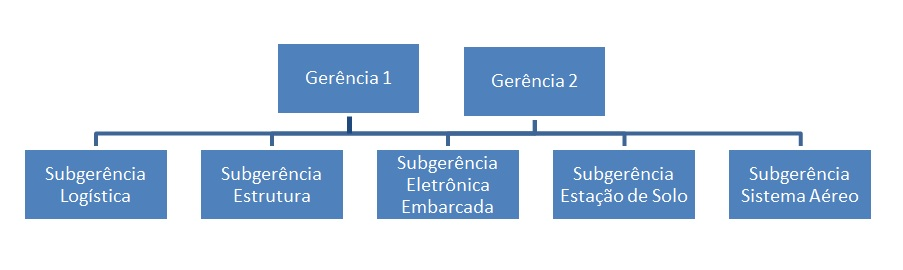
\includegraphics[width=0.6\textwidth]{figuras/eap}
  	\caption{Divisão de gerência e subgerência}
  	\label{img:eap}
  \end{figure}

  Os integrantes do grupo escolheram as áreas que melhor se identificaram para desenvolver as pesquisas ao longo do semestre. Dentre estes, dois foram designados gerentes gerais e outros cinco subgerentes das grandes áreas de pesquisa.

  A dinâmica entre os gerentes e os subgerentes foi desenvolvida de maneira com que todas as partes estejam integradas. Alguns requisitos foram estabelecidos para melhor comunicação entre todos os integrantes do projeto:

  \begin{itemize}
    \item Todas as demandas de grupo deverão ser discutidas nas reuniões em horários de aula com a presença de todos os integrantes do grupo.
    \item As avaliações serão individuais: com o auxílio de uma planilha, os subgerentes deverão avaliar os integrantes do grupo, bem como a gerência geral.
    \item A gerência geral deverá avaliar todos os integrantes do projeto.
    \item Reuniões semanais, além das reuniões em horários de aula,com a presença de todos ou apenas subgerência, com frequência mínima de uma por semana.
    \item Cada subgerente terá a liberdade de desenvolver a dinâmica de grupo que melhor se adequar às necessidades da pesquisa. Contudo, a dinâmica de projeto será a mesma.
    \item As avaliações individuais supracitadas serão feitas ao final de cada etapa, ponto de controle, e serão avaliados:
    \item Pontualidade na entrega de atividades: é importante para manter os prazos de entrega da disciplina e para não sobrecarregar outros integrantes.
    \item Assiduidade nas reuniões: é importante que todos os integrantes estejam presentes nas reuniões estabelecidas, pois a interação destes com o conteúdo discutido é fator sine qua non para a melhor qualidade das pesquisas e compreensão das dificuldades do projeto.
    \item Conteúdo da pesquisa: fontes bibliográficas confiáveis, concordância no desenvolvimento do tópico.
  \end{itemize}

\section{Cronograma}

As atividades para desenvolvimento do projeto SUM, do grupo 1, da disciplina Projeto Integrador 1 deverão ser divididas em etapas, que serão avaliadas nos pontos de controle um, dois e três.

Os cronogramas a seguir apresentam como serão organizadas e direcionadas  as tarefas e atividades para elaboração de relatórios para apresentação nos pontos de controle da disciplina. As atividades serão desenvolvidas durante o semestre (tabelas \ref{tab:cronograma1}, \ref{tab:cronograma2} e \ref{tab:cronograma3}) com a organização datada nos mesmos.

Ao início de cada Ponto de Controle, todos os integrantes devem elaborar uma revisão bibliográfica, ou complementar a anterior, sobre o novo conteúdo a ser desenvolvido e avaliado pelos professores da disciplina. O prazo para a sua elaboração será, sempre que possível, no período de quatro dias. E, com as informações coletadas, seguem as atividades propostas para a elaboração do relatório.

Na quinta-feira anterior ao dia de apresentação do Ponto de Controle, o relatório preliminar deverá ser entregue ao professor orientador para uma revisão geral. Após as correções feitas pelos anos,  o relatório poderá  ser entregue via \textit{Moodle}.

\begin{table}[H]
\centering
\begin{tabular}{|p{2.5cm}|p{0.5cm}|p{0.5cm}|p{0.5cm}|p{0.5cm}|p{0.5cm}|p{0.5cm}|p{0.5cm}|p{0.5cm}|p{0.5cm}|p{0.5cm}|p{0.5cm}|p{0.5cm}|p{0.5cm}|p{0.5cm}|p{0.5cm}|}
\hline
\multicolumn{16}{|c|}{Primeiro ponto de controle}                                                                                                                                                                                                                                                                                                                                                                          \\ \hline
Atividades                     & \scalebox{.7}{21/09}                     & \scalebox{.7}{22/09}                     & \scalebox{.7}{23/09}                     & \scalebox{.7}{24/09}                     & \scalebox{.7}{25/09}                     & \scalebox{.7}{26/09}                     & \scalebox{.7}{27/09}                     & \scalebox{.7}{28/09}                     & \scalebox{.7}{29/09}                     & \scalebox{.7}{30/09}                     & \scalebox{.7}{01/10}                     & \scalebox{.7}{02/10}                     & \scalebox{.7}{03/10} & \scalebox{.7}{04/10} & \scalebox{.7}{05/10}                     \\ \hline
Revisão bibliográfica          & \cellcolor[HTML]{3166FF}X & \cellcolor[HTML]{3166FF}X & \cellcolor[HTML]{3166FF}X & \cellcolor[HTML]{3166FF}X &                           &                           &                           &                           &                           &                           &                           &                           &       &       &                           \\ \hline
Definição escopo               &                           &                           &                           &                           & \cellcolor[HTML]{3166FF}X &                           &                           &                           &                           &                           &                           &                           &       &       &                           \\ \hline
Revisão 1.0                    &                           &                           &                           &                           & \cellcolor[HTML]{3166FF}X &                           &                           &                           &                           &                           &                           &                           &       &       &                           \\ \hline
Latex                          &                           &                           &                           &                           & \cellcolor[HTML]{3166FF}X & \cellcolor[HTML]{3166FF}X & \cellcolor[HTML]{3166FF}X &                           &                           &                           &                           &                           &       &       &                           \\ \hline
Apresentação 1.0               &                           &                           &                           &                           &                           &                           &                           & \cellcolor[HTML]{3166FF}X &                           &                           &                           &                           &       &       &                           \\ \hline
Revisão 2.0                    &                           &                           &                           &                           &                           &                           &                           & \cellcolor[HTML]{3166FF}X & \cellcolor[HTML]{3166FF}X & \cellcolor[HTML]{3166FF}X & \cellcolor[HTML]{3166FF}X &                           &       &       &                           \\ \hline
Revisão professor              &                           &                           &                           &                           &                           &                           &                           &                           &                           &                           & \cellcolor[HTML]{3166FF}X & \cellcolor[HTML]{3166FF}X &       &       &                           \\ \hline
Revisão 3.0                    &                           &                           &                           &                           &                           &                           &                           &                           &                           &                           &                           & \cellcolor[HTML]{3166FF}X &       &       &                           \\ \hline
Apresentação ponto de controle &                           &                           &                           &                           &                           &                           &                           &                           &                           &                           &                           &                           &       &       & \cellcolor[HTML]{3166FF}X \\ \hline
\end{tabular}
\caption{Cronograma de atividades até o primeiro Ponto de Controle de PI 1.}
\label{tab:cronograma1}
\end{table}

    \begin{table}[H]
    \centering
    \begin{tabular}{|p{2.5cm}|p{0.5cm}|p{0.5cm}|p{0.5cm}|p{0.5cm}|p{0.5cm}|p{0.5cm}|p{0.5cm}|p{0.5cm}|p{0.5cm}|p{0.5cm}|p{0.5cm}|p{0.5cm}|p{0.5cm}|p{0.5cm}|p{0.5cm}|}
    \hline
    \multicolumn{16}{|c|}{Segundo ponto de controle}                                                                                                                                                                                                                                                                                                                                                                                                                                                    \\ \hline
    Atividades                                                      & \scalebox{.7}{12/10}                     & \scalebox{.7}{13/10}                     & \scalebox{.7}{14/10}                     & \scalebox{.7}{15/10}                     & \scalebox{.7}{16/10}                     & \scalebox{.7}{17/10}                     & \scalebox{.7}{18/10}                     & \scalebox{.7}{19/10}                     & \scalebox{.7}{20/10}                     & \scalebox{.7}{21/10}                     & \scalebox{.7}{22/10}                     & \scalebox{.7}{23/10}                     & \scalebox{.7}{29/10}                     & \scalebox{.7}{30/10}                     & \scalebox{.7}{04/11}                     \\ \hline
    Revisão bibliográfica                                           & \cellcolor[HTML]{3166FF}X & \cellcolor[HTML]{3166FF}X & \cellcolor[HTML]{3166FF}X & \cellcolor[HTML]{3166FF}X &                           &                           &                           &                           &                           &                           &                           &                           &                           &                           &                           \\ \hline
    Aprimoramento de aspectos técnicos                              &                           &                           &                           & \cellcolor[HTML]{3166FF}X & \cellcolor[HTML]{3166FF}X & \cellcolor[HTML]{3166FF}X &                           &                           &                           &                           &                           &                           &                           &                           &                           \\ \hline
    Elaboração de simulação Catia                                   &                           &                           & \cellcolor[HTML]{3166FF}X & \cellcolor[HTML]{3166FF}X & \cellcolor[HTML]{3166FF}X & \cellcolor[HTML]{3166FF}X & \cellcolor[HTML]{3166FF}X & \cellcolor[HTML]{3166FF}X &                           &                           &                           &                           &                           &                           &                           \\ \hline
    Qualidade das justificativa das escolhas (quadros comparativos) &                           &                           &                           &                           &                           &                           &                           &                           & \cellcolor[HTML]{3166FF}X & \cellcolor[HTML]{3166FF}X & \cellcolor[HTML]{3166FF}X &                           &                           &                           &                           \\ \hline
    Revisão 1.0                                                     &                           &                           &                           &                           &                           &                           &                           &                           &                           &                           &                           & \cellcolor[HTML]{3166FF}X &                           &                           &                           \\ \hline
    Revisão professor                                               &                           &                           &                           &                           &                           &                           &                           &                           &                           &                           &                           &                           & \cellcolor[HTML]{3166FF}X &                           &                           \\ \hline
    Revisão 2.0                                                     &                           &                           &                           &                           &                           &                           &                           &                           &                           &                           &                           &                           & \cellcolor[HTML]{3166FF}X & \cellcolor[HTML]{3166FF}X &                           \\ \hline
    Apresentação ponto de controle                                  &                           &                           &                           &                           &                           &                           &                           &                           &                           &                           &                           &                           &                           &                           & \cellcolor[HTML]{3166FF}X \\ \hline
    \end{tabular}
  \caption{Cronograma de atividades para o segundo  Ponto de Controle de PI 1.}
  \label{tab:cronograma2}
    \end{table}

\begin{table}[H]
\centering
  \begin{tabular}{|p{2.5cm}|p{0.5cm}|p{0.5cm}|p{0.5cm}|p{0.5cm}|p{0.5cm}|p{0.5cm}|p{0.5cm}|p{0.5cm}|p{0.5cm}|p{0.5cm}|p{0.5cm}|p{0.5cm}|p{0.5cm}|p{0.5cm}|p{0.5cm}|}
\hline
\multicolumn{16}{|c|}{Terceiro ponto de controle}                                                                                                                                                                                                                                                                                                                                                                 \\ \hline
Atividades            & \scalebox{.7}{11/11}                     & \scalebox{.7}{12/11}                     & \scalebox{.7}{13/11}                     & \scalebox{.7}{14/11}                     & \scalebox{.7}{15/11}                     & \scalebox{.7}{16/11}                     & \scalebox{.7}{17/11}                     & \scalebox{.7}{18/11}                     & \scalebox{.7}{19/11}                     & \scalebox{.7}{20/11}                     & \scalebox{.7}{21/11}                     & \scalebox{.7}{22/11} & \scalebox{.7}{25/11}                     & \scalebox{.7}{27/11} & \scalebox{.7}{30/11}                     \\ \hline
Revisão bibliográfica & \cellcolor[HTML]{FE0000}X & \cellcolor[HTML]{FE0000}X & \cellcolor[HTML]{FE0000}X & \cellcolor[HTML]{FE0000}X &                           &                           &                           &                           &                           &                           &                           &       &                           &       &                           \\ \hline
Relação de custo      &                           &                           &                           & \cellcolor[HTML]{FE0000}X & \cellcolor[HTML]{FE0000}X & \cellcolor[HTML]{FE0000}X &                           &                           &                           &                           &                           &       &                           &       &                           \\ \hline
Viabilidade econômica &                           &                           &                           &                           &                           & \cellcolor[HTML]{FE0000}X & \cellcolor[HTML]{FE0000}X & \cellcolor[HTML]{FE0000}X & \cellcolor[HTML]{FE0000}X &                           &                           &       &                           &       &                           \\ \hline
Revisão               &                           &                           &                           &                           &                           &                           &                           &                           &                           & \cellcolor[HTML]{FE0000}X & \cellcolor[HTML]{FE0000}X &       &                           &       &                           \\ \hline
Revisão professor     &                           &                           &                           &                           &                           &                           &                           &                           &                           &                           &                           &       & \cellcolor[HTML]{FE0000}X &       &                           \\ \hline
Revisão final         &                           &                           &                           &                           &                           &                           &                           &                           &                           &                           &                           &       &                           &       & \cellcolor[HTML]{FE0000}X \\ \hline
Apresentação final    &                           &                           &                           &                           &                           &                           &                           &                           &                           &                           &                           &       &                           &       & \cellcolor[HTML]{FE0000}X \\ \hline
\end{tabular}

  \caption{Cronograma de atividades para o terceiro  Ponto de Controle de PI 1.}
  \label{tab:cronograma3}
\end{table}

\noindent \textbf{Legenda:} \\
\crule[red]{0.5cm}{0.3cm}	Atividade realizada \\
\crule[blue]{0.5cm}{0.3cm} Atividade não realizada \\

\section{Organização do Documento} % (fold)
\label{sec:organiza_o_do_documento}

  O relatório do Ponto de Controle 2 da disciplina de Projeto Integrador 1 do grupo 1 irá abordar, além da definição do escopo do projeto do SUM, o desenvolvimento técnico do sistema do balão de acordo com as grandes áreas de pesquisas definidas na EAP.

  O primeiro tópico do desenvolvimento será a proposição de um modelo geral do Sistema Unificado de Monitoramento, explanando de maneira simplificada o seu funcionamento, de modo que o leitor consiga acompanhar os tópicos seguintes referentes à estrutura e sistema aéreo, estação de solo, eletrônica embarcada e consumo energético.

  O tópico Subprojeto de Estrutura e Sistema Aéreo apresenta e desenvolve modelos matemáticos aplicados à estrutura do balão cativo, materiais e gás a serem utilizados, bem como os cálculos de volume do balão, empuxo líquido e forças atuantes. O posicionamento dos cabos e a sustentação do mesmo também são

  O Subprojeto da Estação de Solo apresenta os dados sobre armazenamento e processamento de imagens, as configurações dos servidores, como será a comunicação  do operador da estação com a segurança do campus, a localização da estação de solo.

  As configurações das câmeras e dos sensores, establização da carga útil em casos de condições climáticas desfavoráveis, manutenção do balão e integração das soluções de hardware e software estão dispostas no Subprojeto de Eletrônica Embarcada.

  A análise de melhor opção para alimentação energética do SUM, os dados referentes ao consumo e os diagramas do processo de fornecimento energético estão dispostos no subtópico Consumo Energético.

  A integração de todas as grandes áreas de pesquisa e do conteúdo desenvolvido estará no subtópico Integração da Solução, apresentando de maneira técnica todo o funcionamento dos balões cativos, para, por fim, concluir o relatório com os dados e avaliações preliminares.
